Let's consider the algorithm described in the question with pools of $k$ persons. The probability for a given person to be positive is p and all people are considered to have independent behaviour. Therefore we can compute the probability for a test on a pool on k people to be negative.

$\mathcal{P}(test\ negative\ for\ k\ persons) = (1-p)^{k}$

When we are testing a pool there are only two cases :
\begin{itemize}
	\item the test on the pool is negative and we are done ; we do only one test
	\item the test on the pool is positive and we need to test each individual of the pool ; we do $k+1$ tests.
\end{itemize}

We are now able to compute the expected number of tests to be performed on a pool of k people :

$\mathbb{E}(number\ of\ tests\ on\ a\ pool) = [1-(1-p)^{k}](k+1)+(1-p)^{k} = -k(1-p)^{k}+k+1$

We have $n/k$ pools of k people. So the total number of tests is :

$T = (n/k) \mathbb{E}(number\ of\ tests\ on\ a\ pool) = -n(1-p)^{k} + n(1+1/k)$

$T/n = -(1-p)^{k} + 1/k+1$

To simplify the computations, let's consider the function g such that :

$T/n = g(k) + 1$ with $g(k) = -(1-p)^{k}+1/k$

Find the best k possible is equivalent to find the minimum of the function g. Doing it an analytical way (by trying to find the minimum of the derivative) is difficult but to compute the minimum of g we can use a numerical approach such as gradient descent.

\begin{figure}[H]
\begin{center}
   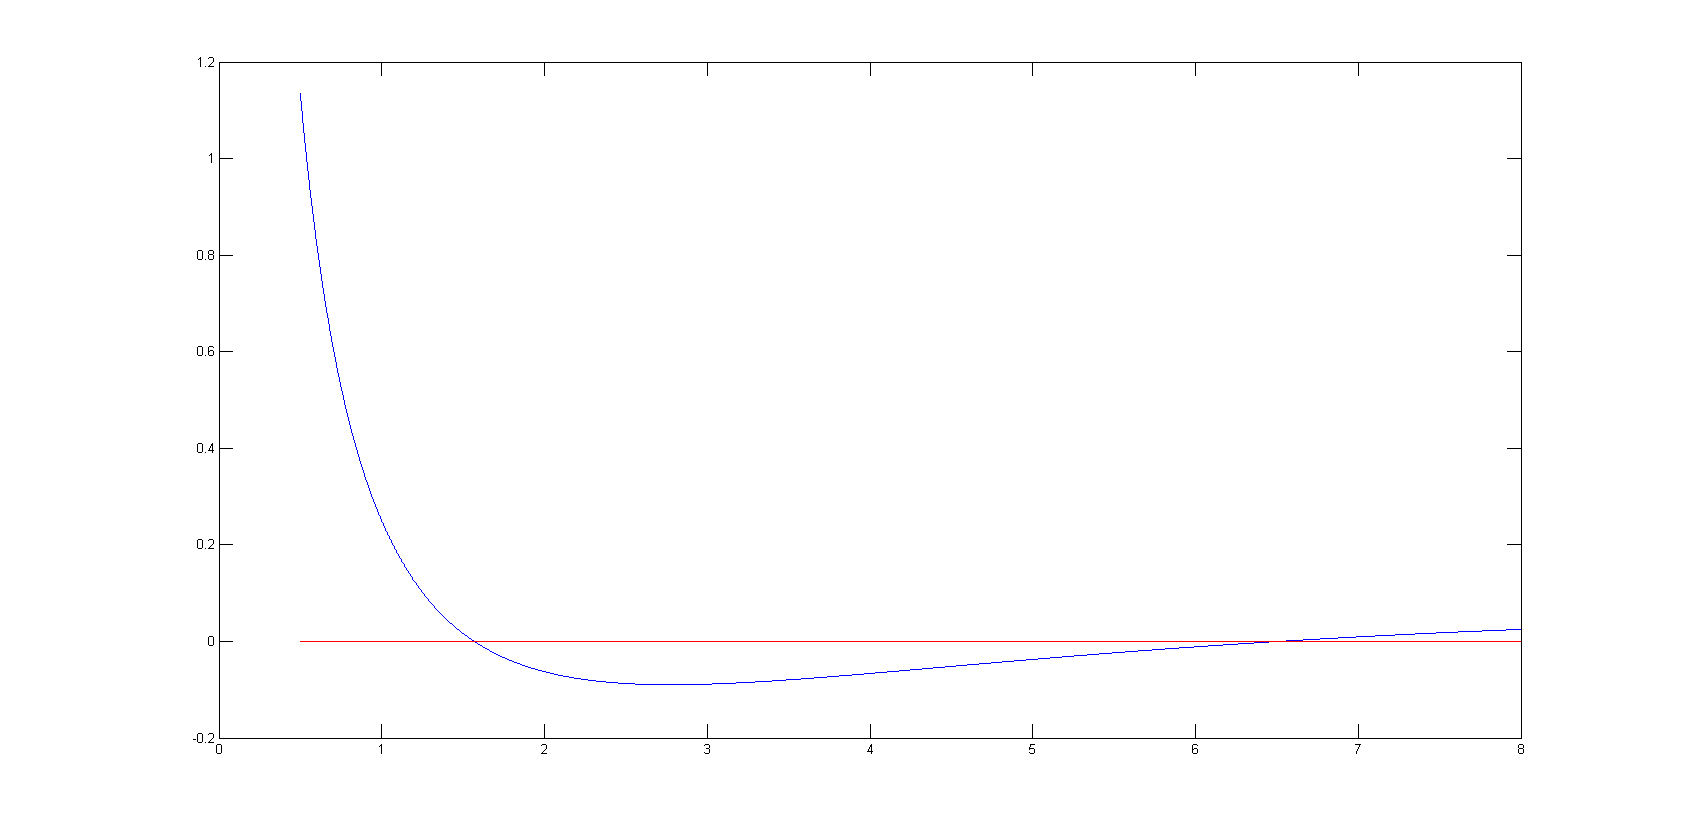
\includegraphics[height=8cm]{fig5.png}
	\caption{plot of g(k) for p = 0.25}
	\label{plot}
	\end{center}
\end{figure}

\paragraph{}
This way of pooling blood is more efficient than testing everybody if and only if $T/n<1$, i.e. $\exists k \geqslant 2$ such that $g(k)<0$. 
By doing a numerical simulation on the function g, we can show that there exists such an integer k if and only if $p<1/2$. Therefore, this way of pooling blood is more efficient than testing everybody if $p<1/2$.


\paragraph{}
Nevertheless, the algorithm introduced here is not the more efficient for group testing and we won't show it here but an approach by dichotomy where we test the two halves of a pool when the test is positive is always profitable if $p<1$.